\section{Lists with no correct choice}
\label{app:abstention}
We build the lists with no correct choice from examples with any number of correct choices and leave out every correct choice. A list holds either random choices from the dataset that are not in the example's list, or the example's own distractors. We send each list without and with a ``none of the above'' choice. Without it, we report the confidence of the prediction. With it, ``none of the above'' is the only correct answer, and we report the share of predictions that select it.

Without a ``none of the above'' choice, the mean confidence is 0.49 to 0.71 on HotpotQA and 0.74 to 0.87 on MetaTool and ECtHR (Table~\ref{tab:abstention}). With it, the models select it in 93\% to 100\% of the lists of random choices and in 79\% to 88\% of the HotpotQA lists of the example's own distractors, and in 7\% to 37\% of the ECtHR lists (Table~\ref{tab:nota}).

% Figure~\ref{fig:exact-set} belongs to Appendix~\ref{app:thresholds}. It is set here to print on the page of that appendix.
\begin{figure*}[t]
\centering
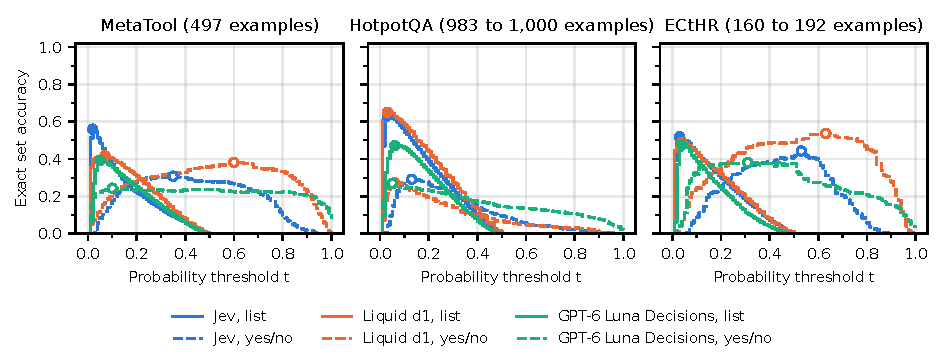
\includegraphics[width=\linewidth]{figures/exact_set}
\caption{Exact set accuracy: the share of examples in which every correct choice is at or above the threshold $t$ and every distractor is below it. Above 0.50 the list curves are 0 by construction.}
\label{fig:exact-set}
\end{figure*}

\begin{table}[H]
\caption{Mean confidence on the answered lists with no correct choice and no ``none of the above'' choice (\emph{Conf.}). Appendix~\ref{app:refusals} counts the refused lists.}
\label{tab:abstention}
\centering
\resizebox{\linewidth}{!}{\begin{tabular}{lrrrrrrrrrr}
\toprule
 & \multicolumn{4}{c}{5 random options} & \multicolumn{6}{c}{Options of the example, none correct} \\
\cmidrule(lr){2-5} \cmidrule(lr){6-11}
 & \multicolumn{2}{c}{MetaTool} & \multicolumn{2}{c}{HotpotQA} & \multicolumn{2}{c}{MetaTool} & \multicolumn{2}{c}{HotpotQA} & \multicolumn{2}{c}{ECtHR} \\
\cmidrule(lr){2-3} \cmidrule(lr){4-5} \cmidrule(lr){6-7} \cmidrule(lr){8-9} \cmidrule(lr){10-11}
Model & Refused & Conf. & Refused & Conf. & Refused & Conf. & Refused & Conf. & Refused & Conf. \\
\midrule
Jev & 0\% & 0.78 & 0\% & 0.58 & 0\% & 0.80 & 0\% & 0.61 & 0\% & 0.83 \\
Liquid d1 & 0\% & 0.74 & 0\% & 0.49 & 0\% & 0.77 & 0\% & 0.67 & 0\% & 0.87 \\
GPT-6 Luna Decisions & 58\% & 0.79 & 98\% & 0.71 & 23\% & 0.78 & 27\% & 0.65 & 1\% & 0.87 \\
\bottomrule
\end{tabular}
}
\end{table}

\begin{table}[H]
\caption{Share of predictions that select ``none of the above'', the only correct choice (\emph{Selected}).}
\label{tab:nota}
\centering
\resizebox{\linewidth}{!}{\begin{tabular}{lrrrr}
\toprule
 & \multicolumn{2}{c}{Random choices} & \multicolumn{2}{c}{The example's own} \\
\cmidrule(lr){2-3} \cmidrule(lr){4-5}
 & \multicolumn{1}{c}{MetaTool} & \multicolumn{1}{c}{HotpotQA} & \multicolumn{1}{c}{HotpotQA} & \multicolumn{1}{c}{ECtHR} \\
\cmidrule(lr){2-2} \cmidrule(lr){3-3} \cmidrule(lr){4-4} \cmidrule(lr){5-5}
Model & Selected & Selected & Selected & Selected \\
\midrule
Jev & 95\% & 100\% & 84\% & 37\% \\
Liquid d1 & 98\% & 100\% & 88\% & 7\% \\
GPT-6 Luna Decisions & 93\% & 100\% & 79\% & 17\% \\
\bottomrule
\end{tabular}
}
\end{table}
